\subsection{Radio-Layer Protocol Sensitivity}
\label{sec:res:radio}

Table~\ref{tab:radio} compares a random and a group-disjoint split on the radio layer of \DA{}, with the 30 capture sessions or the 42 experiment runs as groups; a third protocol, which keeps every attack category on both sides, gives the same picture (repository). Grouped by sessions, a random split raises macro-$F_1$ over a group-disjoint split by \RRadSessMin{} to \RRadSessMax{} across the six architectures, \RRadSessAvg{} on average. This gain is not statistically significant: the corrected interval of the average gain is \RRadSessLo{} to \RRadSessHi{} ($p = \RRadSessP$), and no architecture's gain is significant after Holm correction. Grouped by runs, the average gain is \RRadRunAvg{}, with a corrected interval of \RRadRunLo{} to \RRadRunHi{} ($p = \RRadRunP$), and again no architecture's gain is significant after Holm correction. The input-blind baselines gain nothing under either grouping, so class composition does not move macro-$F_1$ between protocols. A model-free probe is consistent with recognition of capture groups: under a random split, \RRadNNSame\% of the test windows have their nearest training window in the same session, although windows share no records, and a one-nearest-neighbor lookup reaches a macro-$F_1$ of \RRadNNRand{}, against \RRadNNGd{} under a session-disjoint split. The probe shows that recognizing the group is available to a model, not that the trained models rely on it.

\begin{table}[t]
\caption{Radio-layer protocol sensitivity on \DA{}: macro-$F_1$ under a random (R) and a group-disjoint (GD) split, with sessions (30 groups) or runs (42 groups) as the group, and the gain of the random split with its Nadeau--Bengio corrected 95\% interval (group counts), over 20 splits with two model seeds each. Intervals are unadjusted; $^{\ast}$: significant after Holm correction across the six architectures.}
\label{tab:radio}
\centering
\scriptsize
\setlength{\tabcolsep}{2.2pt}
\begin{tabular}{lcccccc}
\toprule
 & \multicolumn{3}{c}{30 sessions} & \multicolumn{3}{c}{42 runs} \\
\cmidrule(lr){2-4}\cmidrule(lr){5-7}
Model & R & GD & Gain [95\% CI] & R & GD & Gain [95\% CI] \\
\midrule
LR & 0.836 & 0.744 & +0.093 [$-$0.08, 0.26] & 0.834 & 0.738 & +0.096 [$-$0.08, 0.28] \\
DT & 0.950 & 0.782 & +0.168 [$-$0.01, 0.35] & 0.945 & 0.752 & +0.193 [0.02, 0.36] \\
RF & 0.970 & 0.853 & +0.117 [$-$0.07, 0.30] & 0.970 & 0.816 & +0.154 [$-$0.04, 0.35] \\
XGB & 0.977 & 0.836 & +0.141 [$-$0.03, 0.32] & 0.979 & 0.813 & +0.166 [$-$0.02, 0.35] \\
HGB & 0.982 & 0.844 & +0.138 [$-$0.03, 0.31] & 0.983 & 0.816 & +0.167 [$-$0.02, 0.35] \\
MLP & 0.954 & 0.828 & +0.126 [$-$0.04, 0.29] & 0.955 & 0.814 & +0.141 [$-$0.03, 0.31] \\
\textit{Strat.} & 0.498 & 0.507 & $-$0.009 [$-$0.02, 0.00] & 0.497 & 0.507 & $-$0.010 [$-$0.02, 0.00] \\
\textit{Maj.} & 0.431 & 0.434 & $-$0.002 [$-$0.02, 0.02] & 0.431 & 0.434 & $-$0.003 [$-$0.02, 0.01] \\
\midrule
Average &  &  & +0.131 [$-$0.03, 0.30] &  &  & +0.153 [$-$0.02, 0.33] \\
\bottomrule
\end{tabular}

\end{table}

The radio layer cannot support operating figures. It holds \RRadBenignWin{} benign windows, about \RRadBenignHours{} hours of data, recorded mostly with one UE and, for nine of the ten benign sessions, six weeks before the first attack session. When each benign session is held out alone (Fig.~\ref{fig:benign}), the false positive rate averaged over the six architectures is at most \BenLowMax{} for \BenLowN{} sessions and \BenHighMin{} to \BenHighMax{} for sessions \BenHighSessions{}, and a bootstrap over splits and sessions puts the pooled false positive rate between \RadCbFPRlo{} and \RadCbFPRhi{} (lowest and highest interval bound across architectures). A false positive rate this dependent on which benign session a detector meets cannot be turned into an alert rate for another network, so we report none for the radio layer.

\begin{figure}[t]
\centering
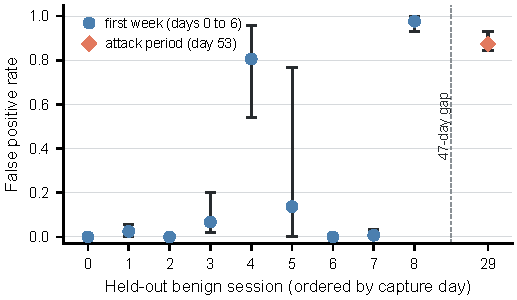
\includegraphics[width=\columnwidth]{figs/fig_benign}
\caption{False positive rate on each benign radio session of \DA{} when that session alone is held out and the models train on the other 29: mean (marker) and range (bar) over the six architectures, sessions in capture order. Within one week of capture, sessions range from no false positives to almost every window flagged, so the radio layer supports no operating figure.}
\label{fig:benign}
\end{figure}

\subsection{Decision Latency of Window-Level Detectors}
\label{sec:res:latency}

We measured latency separately, for window-level detectors only, and it is not part of the test. Our C xApp in FlexRIC v2.0.0 subscribes to E2SM-KPM reports from FlexRIC's emulated gNB over SCTP, with 16 measurement items per UE, scores every UE of a report with ONNX Runtime, answers each report with one E2SM-RC control message, and waits for the acknowledgment. The emulated node reports synthetic values, so the xApp scores held-out radio test windows in their place; the C code reproduced the Python scores on all 589 test windows to within $4\times10^{-7}$. With a report every 10\,ms (\RicNten{} reports per model), the full loop from report to acknowledged control message takes \RicLoopTenPnnMin{} to \RicLoopTenPnnMax{}\,ms at the 99th percentile over the six models (Table~\ref{tab:ric}). Delivery and control account for at least \RicTransportShareMin\% of the mean loop time, and inference takes at most \RicInfTenPnnMax{}\,ms at the 99th percentile, so once a RIC is in the path the model barely matters. At a 1\,ms period the loop ran faster (\RicLoopOnePnnMin{} to \RicLoopOnePnnMax{}\,ms), which fits a host that idles between sparse reports and pays to wake up: these are processing costs of the RIC software path on one host, under WSL2, without CPU isolation and with synthetic measurements over loopback, not the delay of a deployment.

Two limits follow. First, computation is not what limits a window-level detector: it decides once its 16\,s window is complete, so a compute tail of a few milliseconds is small next to the detection delay. Second, we have no measured latency for flow-level detectors: their records need a transport to the xApp that our loop lacks and O-RAN does not define, and the cost of a native user-plane exporter is unknown. We therefore make no latency claim for flow detectors.

\begin{table}[t]
\caption{Decision loop of a window-level detector through FlexRIC with an emulated E2 node on one host, in ms, ranges over models (one trained model per architecture, split seed 101), at a 10\,ms reporting period (six models, \RicNten{} reports each) or a 1\,ms period (LR and RF, \RicNone{} reports each). Terms of Eq.~\eqref{eq:latency}: delivery to the xApp ($t_{\mathrm{ind}}$), queueing ($t_{q}$), aggregation ($t_{\mathrm{feat}}$) and inference ($t_{\mathrm{inf}}$) for one UE, and control up to acknowledgment ($t_{\mathrm{act}}$). ``Loop'': KPM header timestamp to acknowledgment, for the first UE of a report or all its UEs.}
\label{tab:ric}
\centering
\scriptsize
\setlength{\tabcolsep}{2.4pt}
% GENERATED by analysis/make_tables.py on 2026-09-26
% source: EXP-061 ric_latency
% commit: 30327c2
% DO NOT EDIT. Edit the generator, then re-run `make tables`.
\begin{tabular}{lcccc}
\toprule
& \multicolumn{2}{c}{10\,ms, six models} & \multicolumn{2}{c}{1\,ms, LR and RF} \\
Term & $p_{50}$ & $p_{99}$ & $p_{50}$ & $p_{99}$ \\
\midrule
$t_{\mathrm{ind}}$ & 1.51--1.86 & 3.02--3.05 & 0.51--0.53 & 0.84--0.98 \\
$t_{q}$ & 0.063--0.071 & 0.18--0.21 & 0.015--0.016 & 0.069 \\
$t_{\mathrm{feat}}$ & 0.001 & 0.002--0.003 & $<$0.001 & 0.001 \\
$t_{\mathrm{inf}}$ & 0.050--0.12 & 0.13--0.23 & 0.014--0.025 & 0.038--0.050 \\
$t_{\mathrm{act}}$ & 0.72--0.87 & 1.40--1.50 & 0.20--0.21 & 0.53--0.60 \\
\midrule
Loop, 1 UE & 2.38--2.97 & 4.36--4.59 & 0.76--0.79 & 1.38--1.59 \\
Loop, all & 2.48--3.18 & 4.45--4.95 & 0.77--0.86 & 1.42--1.69 \\
\bottomrule
\end{tabular}

\end{table}
